\documentclass[a4paper]{article}

% This is a simple document with examples figures, equations and tables. 
% It was adapted from earlier templates made by writelatex (the precursor of overleaf)
% This particular version was adapted by Simon M. Mudd on 09-Feb-2022
% If you want to learn more about latex use this link: https://www.overleaf.com/learn/latex/Learn_LaTeX_in_30_minutes

% In latex any line that has a % in front is a comment and won't appear in the document. 

% You can add packages here. These can give you some nice formatting tools. 
% But I wouldn't mess about with this until you have more experience with latex
\usepackage[english]{babel}
\usepackage[utf8]{inputenc}
\usepackage{amsmath}
\usepackage{graphicx}
\usepackage{float}
\usepackage{natbib}

% Here is where you can set the font
% the first line just say to load the package that allows you to input fonts
% the second is the actual font. 
% You can choose a font from here: https://www.overleaf.com/learn/latex/Font_typefaces
% and put the name in the curly brackets on the second line below
\usepackage[T1]{fontenc}
\usepackage{lmodern}


\title{Your Paper}

\author{Write your name here}

\date{\today}

\begin{document}
\maketitle

% You can change the citation style here
% Here is a place to find out the options: https://gking.harvard.edu/files/natnotes2.pdf
\setcitestyle{round,aysep={,},yysep={;}}

% If you don't want an abstract just put % symbols in front of the three lines below this one. 
\begin{abstract}
Your abstract.
\end{abstract}

\section{Introduction}

Your introduction goes here. 

\section{Some Examples}
\label{sec:examples}

Here is a section where I refer to a section header. This section is Section \ref{sec:examples}. You use the ``ref'' command as a reference so you don't actually need to remember any numbers. Whenever you update your sections the numbering will be updated as well. 

\subsection{How to Make Sections and Subsections}

Use section and subsection commands to organize your document. \LaTeX{} handles all the formatting and numbering automatically. Use ref and label commands for cross-references.

\subsubsection{You can nest sections with lots of sub commands}

You could even do a ``subsubsubsection'' but I'm not sure why you would want to do that. Just for fun here is a reference to the conclusions section, which is Section~\ref{sec:conclusions}.

\subsection{Citing and references}

You can cite things with various commands but the two ones to remember are citep and citet. citep is your normal citing method and citep is when you want to include the author name in the text. An example of citep is this one \citep{gilbert_geology_1877}. If you want to cite \citet{morisawa_quantitative_1962} in line with the text you use the command ``citet''. This is an example of a paper with multiple authors \citep{clubb_differences_2020}. And here is an example with mulitple papers \citep{clubb_differences_2020, morisawa_quantitative_1962, gilbert_geology_1877}.

\subsection{How to Include Figures}

First you have to upload the image file (JPEG, PNG or PDF) from your computer to using the upload link the project menu. In this template I put figures into a folder called ``Figures''. Then use the ``includegraphics'' command to include it in your document. You don't really need to remember that, just copy the below stuff after the begin figure line, and then change the filename. Use the figure environment and the caption command to add a number and a caption to your figure. See the code for Figure~\ref{fig:glencoe} in this section for an example.

% Copy this and change the file name to add figures. 
% You can change the size by modifying the width number below
\begin{figure}
\centering
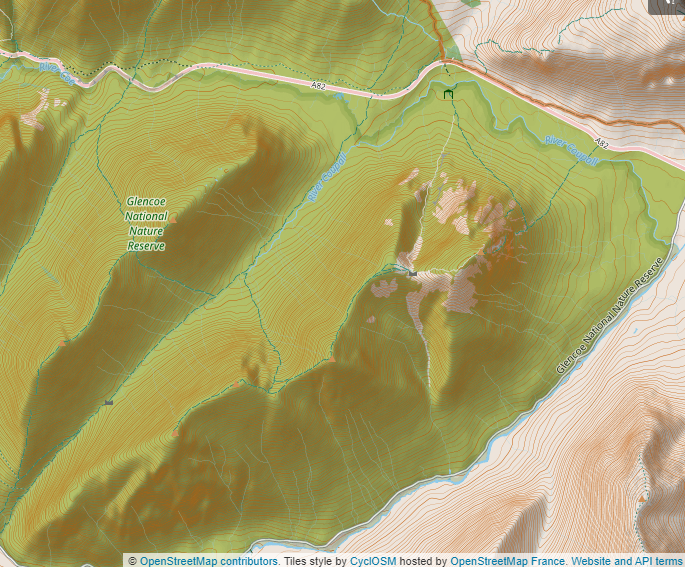
\includegraphics[width=0.8\textwidth]{Figures/glencoe_OSM.png}
\caption{Here is a contour map of Glen Coe from open street maps.}
\label{fig:glencoe}
\end{figure}


\subsection{How to Write Mathematics}

You can use the dollar sign to denote equations, like this: $y = mx+b$. 

You can also use the equation command:

\begin{equation}
\label{eq:decay_equation}
C = P e^x
\end{equation}

Just like sections, tables, and figures, you can label your equations using the ``label'' command and then you don't have to worry about all the numbering. There are many tutorials online about equations in Latex if you are going to do anything complicated. 

If you do use equations in your essays the convention is to use the same format in the text as in the equation, so for example if some symbol in the equation is in italic font then it should be in italic font when you mention it in the text. In latex you can just use the dollar signs on either side of the symbol to give it the same format as the equation. So for example there is a $P$ symbol in equation~\ref{eq:decay_equation}.

\subsection{How to Make Tables}

Use the table and tabular commands for basic tables. I've made an example in Table~\ref{tab:widgets}.

% This is a table. The [H] tells latex to put the table here. 
\begin{table}[H]
\centering
\begin{tabular}{l|r}
Item & Quantity \\\hline
Widgets & 42 \\
Gadgets & 13
\end{tabular}
\caption{An example table.}
\label{tab:widgets}
\end{table}

\section{Conclusions}
\label{sec:conclusions}
Have fun writing documents in overleaf!

% This builds the bibliography
% See https://gking.harvard.edu/files/natnotes2.pdf for options on style
\bibliographystyle{apalike}
\bibliography{bibliography.bib}

\end{document}